% Supplementary material: inclusion criteria, source verification, artifacts, update policy.

\section{Inclusion Criteria, Source Verification, Released Artifacts, and Update Policy}
\label{supp:method}

\subsection{Inclusion Criteria and Appraisal}
\label{subsubsec:intro_screening}

Inclusion criteria for the technique literature were: (T1)~the work concerns models at or below roughly twenty billion parameters, or a compression, adaptation, routing, or deployment technique whose evaluation includes that regime; (T2)~it is a peer-reviewed paper, an archived preprint, or a vendor technical report with a stable identifier; and (T3)~it reports enough methodological detail to determine what was measured.

Inclusion criteria for model variants were: (M1)~a source from the developer (technical report, paper, model card, model repository, or release announcement) that states the parameter count and architecture; (M2)~a public artifact or a documented evaluation card; (M3)~satisfaction of C1, with C2 status recorded separately; and (M4)~a dated release. Fine-tunes and merges of another party's checkpoint were excluded unless their developer released a technical report describing its own training recipe (as for the DeepSeek-R1-Distill models), as were quantized re-uploads, API aliases of a listed checkpoint, and variants differing only in serialization format.

\emph{What is computed and what is decided.} C1, C2, M1, and M4 are computed from recorded fields by \file{apply\_inclusion\_rules.py}: M1 from the stated parameter count and the field \texttt{developer\_source\_found} written by the source check below, and M4 from \texttt{release\_date\_precision}. Three kinds of exclusion are named editorial decisions listed in the script, because they cannot be computed from fields: encoder-decoder architecture (Flan-T5), derivative fine-tunes without a technical report (Nous Hermes~2 Mixtral, Vicuna-7B v1.5, Vicuna-13B, Jan-v1-4B), and an API alias (Mistral Tiny). Records whose size is undisclosed cannot be classified against C1 or C2; all of them, whatever their marketing (for example GPT-4o mini, Amazon Nova Micro and Lite, Claude Haiku, Gemini Flash-Lite, Nex-N2-Mini), are kept in the comparison part of the file with class \texttt{undisclosed} and are neither counted nor plotted as \glspl{slm} or \glspl{llm}. Release dates are recorded at the precision their sources give: day for 174 of the 209 included records, month for 22, and year for 13.

\emph{Appraisal of empirical works.} Works relied on for quantitative claims were appraised on whether they name the harness, state the evaluation conditions, report a matched baseline, and identify the evaluated checkpoint; the outcome, together with the reporting party's independence, is the evidence grade of Section~\ref{subsec:reported_grading}.

\subsection{Source Verification}
\label{subsec:source_verification}

On 8~October 2026, \file{verify\_sources.py} checked every included and excluded record, and every comparison record of stated size, against the Hugging Face Hub API: for each Hub repository a record links, it recorded whether the repository exists, its owner, creation date, licence tag, and the parameter count of its safetensors weights, and it classified the record's reference as a developer page, a paper, a Hub model page, or a secondary source (a model aggregator or press article). The result is written into each record (\texttt{source\_check}, \texttt{developer\_source\_found}) and into \file{source\_check\_log.csv}; Figure~\ref{fig:inventory_pipeline} places the check in the build process. Of the 209 included records, 197 link an existing repository owned by the developer and 12 link the developer's own announcement, paper, or code repository.

The check led to the following corrections, applied by \file{fix\_records\_v3\_6.py} and listed in the file's metadata. Twelve records whose reference was a model aggregator or a press article (the DeepSeek V4 Flash, Ling~3.0 Flash, Laguna, North Mini Code, Inkling Small, Nex-N2-Pro, Dots3-Note Preview, and Granite~4.0 Nano records) were re-sourced to the developer's Hub repository, with the original reference kept as \texttt{discovered\_via}; Ling~3.0 Flash Fin, recorded as API-only, is open-weight under MIT. Ling~3.0 Flash Sante, for which no developer source exists, fails M1 and was excluded. Voxtral Mini, previously excluded as undisclosed with a link to a different model, is the open-weight Voxtral Mini~3B (4.7B including its audio encoder, Apache~2.0) and was included. The BitNet b1.58 record, which described the 2024 paper but linked the 2025 checkpoint, now describes the released 2B4T model. The SmolLM2 records, which linked the SmolLM3 page, the Mistral~7B v0.3 release date (2024, not 2023), and the Granite~4.1 references were corrected. For nine records the ratio of the Hub parameter count to the vendor's nominal size falls outside 0.8--1.25 (for example Gemma~2-2B, nominal 2B, Hub 2.6B; Qwen2.5-Omni-7B, Hub 10.7B including its audio components; BitNet b1.58 2B4T, whose ternary weights are stored packed); the recorded size is the vendor's statement, the Hub count is kept in the log, and none of the differences changes a record's C1 or C2 status.

\begin{figure}[t]
\centering
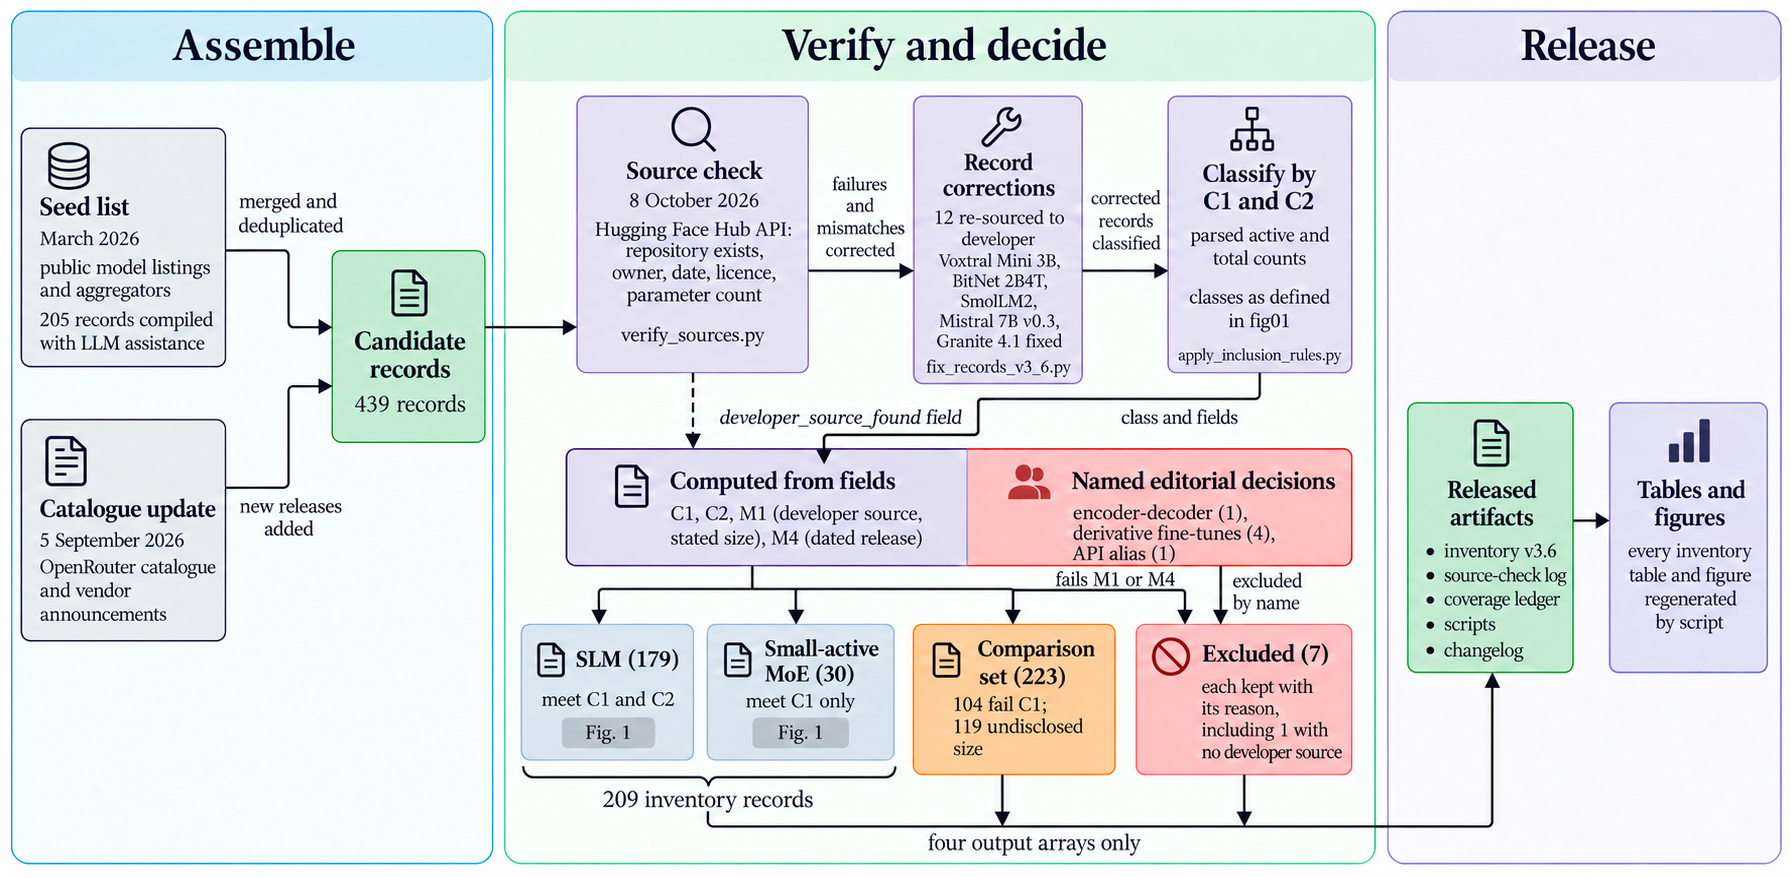
\includegraphics[width=\linewidth]{fig02-inventory-pipeline.png}
\caption{How the inventory was assembled, verified, and filtered. Secondary listings only seeded the candidate list; every record was then checked against its developer source and corrected where needed. C1, C2, M1, and M4 are computed from recorded fields; the encoder-decoder, derivative, and alias exclusions are named editorial decisions. All four arrays, the source-check log, the coverage ledger, the scripts, and the changelog are released.}
\Description{Flow diagram in four columns. Assemble: seed list (March 2026) and catalogue update (September 2026) feed 439 candidate records. Verify: source check against the Hugging Face Hub (October 2026), record corrections, and classification by C1 and C2. Decide: decisions computed from fields, and named editorial exclusions. Arrays: SLM 179, small-active mixture of experts 30, comparison 223 (104 fail C1, 119 undisclosed), and excluded 7. All outputs lead to the released artifacts.}
\label{fig:inventory_pipeline}
\end{figure}

\subsection{Count History}
\label{subsec:count_history}

Earlier drafts reported 126 variants. Version~3.3 of the inventory added 27 releases from May to September 2026 (153). Version~3.4 placed records by the rule rather than by how they had been filed: 64 models meeting C1 had been filed outside the \gls{slm} inventory and two 24B dense models inside it (215). Version~3.5 corrected a parser that had read the total in place of the active count for five legacy \gls{moe} records and removed eleven records by the inclusion criteria (209: 178 \glspl{slm} and 31 small-active-parameter \glspl{moe}). Version~3.6 applied the source verification above: Voxtral Mini~3B entered as an \gls{slm} and Ling~3.0 Flash Sante left, and the four records of undisclosed size that version~3.5 had excluded as ``vendor-positioned small'' were moved to the comparison set with every other undisclosed record (209: 179 \glspl{slm} and 30 small-active-parameter \glspl{moe}; 223 comparison records, of which 104 are of disclosed size and fail C1 and 119 are undisclosed; 7 excluded). The changelog in the released file names every record added, moved, or removed at each step.

\subsection{Released Artifacts}
\label{subsec:intro_artifacts}

The following are released with the paper: the inventory \file{merged\_llm\_database.json} (version~3.6), with one record per variant carrying its parameter counts, C1/C2 status, class, inclusion decision and reason, developer source, source-check result and date, and the excluded and comparison records alongside; the source-check log \file{source\_check\_log.csv}; the audit coverage ledger \file{audit\_coverage\_ledger.csv} (\suppsec~\ref{subsec:audit_ledger}); the scripts that correct and verify records, apply the inclusion rule, build the ledger, and generate every inventory table and figure; and the changelog. They are provided as supplementary files with the submission and will be deposited in a versioned archival repository under a persistent identifier, so that the exact snapshot underlying this paper, and any later one, can be retrieved.

\subsection{Snapshot and Update Policy}
\label{subsubsec:intro_snapshot}

This paper reports model releases through 4~September 2026, as recorded in version~3.6 of the inventory (8~October 2026). Releases appearing between submission and acceptance are added to the released inventory and recorded in the changelog, and are discussed in the text only where they change a conclusion; tables and figures are regenerated from the inventory at the last revision before acceptance. Works appearing during review that bear on RQ2--RQ5 are added to the synthesis, as was done for one study published after the snapshot \citep{laskar2026sftrl}. The released artifact is the authority on what the inventory contained at any given date.
